% Sandia National Laboratories is a multimission laboratory managed and
% operated by National Technology & Engineering Solutions of Sandia, LLC, a
% wholly owned subsidiary of Honeywell International Inc., for the U.S.
% Department of Energy’s National Nuclear Security Administration under
% contract DE-NA0003525.

% Copyright 2002-2022 National Technology & Engineering Solutions of Sandia,
% LLC (NTESS).


\begin{Device}

\symbol
{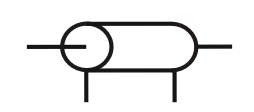
\includegraphics{translineSymbol}}

\device
\begin{alltt}
O<name> <A port (+) node> <A port (-) node>
+ <B port (+) node> <B port (-) node> [model name]
\end{alltt}

\model
\begin{alltt}
.MODEL <model name> LTRA R=<value> L=<value> C=<value>
+ G=<value> LEN=<value> [model parameters]
\end{alltt}

\examples
\begin{alltt}
Oline1 inp inn outp outn cable1
Oline2 inp inn outp outn cable1
\end{alltt}

\comments

The lossy transmission line, or LTRA, device is a two port (\texttt{A}
and \texttt{B}), bi-directional device. The \texttt{(+)} and \texttt{(-)} nodes
define the polarity of a positive voltage at a port.

\texttt{R}, \texttt{L}, \texttt{C}, and \texttt{G} are the resistance,
inductance, capacitance, and conductance of the transmission line per unit
length, respectively. \texttt{LEN} is the total length of the transmission
line. Supported configurations for the LTRA are \texttt{RLC}, \texttt{RC},
\texttt{LC} (lossless) and \texttt{RG}.

The lossy transmission line, or LTRA, device does not work with AC
analysis at this time.  LTRA models will need to be replaced with
lumped transmission line models (YTRANSLINE) when used in AC analysis.
The LTRA models do work correctly in harmonic balance simulation.
\end{Device}


%\paragraph{Device Parameters}
%% This table was generated by Xyce:
%   Xyce -doc O 1
%
\index{lossy transmission line!device instance parameters}
\begin{DeviceParamTableGenerated}{Lossy Transmission Line Device Instance Parameters}{O_1_Device_Instance_Params}
I1 & Initial current at end 1 & A & 0 \\ \hline
I2 & Initial current at end 2 & A & 0 \\ \hline
V1 & Initial voltage at end 1 & V & 0 \\ \hline
V2 & Initial voltage at end 2 & V & 0 \\ \hline
\end{DeviceParamTableGenerated}


\paragraph{Model Parameters}
% This table was generated by Xyce:
%   Xyce -doc O 1
%
\index{lossy transmission line!device model parameters}
\begin{DeviceParamTableGenerated}{Lossy Transmission Line Device Model Parameters}{O_1_Device_Model_Params}
ABS & Abs. rate of change of deriv. for bkpt & -- & 1 \\ \hline
C & Capacitance per unit length & F/m & 0 \\ \hline
COMPACTABS & special abstol for straight line checking & -- & 1e-12 \\ \hline
COMPACTREL & special reltol for straight line checking & -- & 0.001 \\ \hline
COMPLEXSTEPCONTROL & do complex time step control using local truncation error estimation & logical (T/F) & false \\ \hline
G & Conductance per unit length & $\mathsf{\Omega}^{-1}$ m$^{-1}$ & 0 \\ \hline
L & Inductance per unit length & Hm$^{-1}$ & 0 \\ \hline
LEN & length of line & m & 0 \\ \hline
LININTERP & use linear interpolation & logical (T/F) & false \\ \hline
MIXEDINTERP & use linear interpolation if quadratic results look unacceptable & logical (T/F) & false \\ \hline
NOSTEPLIMIT & don't limit timestep size based on the time constant of the line & logical (T/F) & false \\ \hline
QUADINTERP & use quadratic interpolation & logical (T/F) & true \\ \hline
R & Resistance per unit length & $\mathsf{\Omega}/$m & 0 \\ \hline
REL & Rel. rate of change of deriv. for bkpt & -- & 1 \\ \hline
STEPLIMIT & limit timestep size based on the time constant of the line & logical (T/F) & true \\ \hline
TRUNCDONTCUT & don't limit timestep to keep impulse response calculation errors low & logical (T/F) & false \\ \hline
TRUNCNR & use N-R iterations for step calculation in LTRAtrunc & logical (T/F) & false \\ \hline
\end{DeviceParamTableGenerated}


By default time step limiting is on in the LTRA. This means that
simulation step sizes will be reduced if required by the LTRA to
preserve accuracy. This can be disabled by setting
\texttt{NOSTEPLIMIT=1} and \texttt{TRUNCDONTCUT=1} on the
\texttt{.MODEL} line.

The option most worth experimenting with for increasing the speed of
simulation is \texttt{REL}. The default value of 1 is usually safe
from the point of view of accuracy but occasionally increases
computation time. A value greater than 2 eliminates all breakpoints
and may be worth trying depending on the nature of the rest of the
circuit, keeping in mind that it might not be safe from the viewpoint
of accuracy. Breakpoints may be entirely eliminated if the circuit
does not exhibit any sharp discontinuities. Values between 0 and 1 are
usually not required but may be used for setting many breakpoints.

\texttt{COMPACTREL} and \texttt{COMPACTABS} are tolerances that
control when the device should attempt to compact past history. This
can significantly speed up the simulation, and reduce memory usage,
but can negatively impact accuracy and in some cases may cause
problems with the nonlinear solver. In general this capability should
be used with linear type signals, such as square-wave-like
voltages. In order to activate this capability the general device
option \texttt{TRYTOCOMPACT=1} must be set, if it is not no history
compaction will be performed and the \texttt{COMPACT} options will be
ignored.

Example:

\texttt{.OPTIONS DEVICE TRYTOCOMPACT=1}

\paragraph{References}
See references \cite{Roychodhury:1994} and \cite{Spice3f5-user-guide} for more information
about the model.
